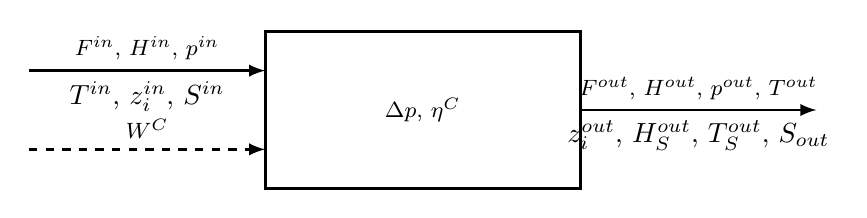
\begin{tikzpicture}[arrow/.style={line width=1pt,->,>=latex}]
	\draw [line width=1pt] (-2,2) rectangle (2,0) node at (0,1) {\footnotesize $\Delta p$, $\eta^C$};
	\draw [arrow] (-5,1.5) -- (-2,1.5) node [pos=0.5, above] {\footnotesize $F^{in}$, $H^{in}$, $p^{in}$} node [pos=0.5, below] {$T^{in}$, $z_i^{in}$, $S^{in}$};
	\draw [line width=1pt,->,>=latex,dashed] (-5,0.5) -- (-2,0.5) node [pos=0.5, above] {\footnotesize $W^C$};
	\draw [arrow] (2,1) -- (5,1) node [pos=0.5, above] {\footnotesize $F^{out}$, $H^{out}$, $p^{out}$, $T^{out}$} node [pos=0.5, below] {$z_i^{out}$, $H_S^{out}$, $T_S^{out}$, $S_{out}$};
\end{tikzpicture}�